% Reconstructed from lecture0.pdf.
% External images and screenshots are intentionally omitted.
% The wording below is preserved from the source deck, including original phrasing.

\documentclass[aspectratio=169,12pt]{beamer}

\usepackage[T1]{fontenc}
\usepackage[utf8]{inputenc}
\usepackage{lmodern}
\usepackage{amsmath,amssymb,mathtools}
\usepackage{tikz}
\usetikzlibrary{arrows.meta,positioning,shapes.geometric}
\usepackage{array}
\usepackage{hyperref}
\usepackage{graphicx}


\definecolor{slideorange}{HTML}{FF5500}
\definecolor{bulletgreen}{HTML}{A8C9A0}
\definecolor{bulletgray}{HTML}{D9E1E8}
\definecolor{warningred}{HTML}{F12A16}
\definecolor{rulegray}{HTML}{C9CED3}

\hypersetup{
  colorlinks=true,
  urlcolor=black,
  linkcolor=black
}
\urlstyle{same}

\setbeamertemplate{navigation symbols}{}
\setbeamercolor{background canvas}{bg=white}
\setbeamercolor{normal text}{fg=black,bg=white}
\setbeamercolor{frametitle}{fg=slideorange,bg=white}
\setbeamercolor{page number in head/foot}{fg=black,bg=white}
\setbeamerfont{frametitle}{series=\bfseries,size=\LARGE}
\setbeamerfont{page number in head/foot}{size=\scriptsize}
\setbeamersize{text margin left=0.85cm,text margin right=0.85cm}

\setbeamertemplate{frametitle}{%
  \vspace*{0.18cm}%
  \begin{beamercolorbox}[wd=\paperwidth,center,sep=0.08cm]{frametitle}
    \usebeamerfont{frametitle}\insertframetitle
  \end{beamercolorbox}%
  \vspace*{0.12cm}%
}

\setbeamertemplate{footline}{%
  \leavevmode
  \begin{beamercolorbox}[wd=\paperwidth,ht=0.42cm,dp=0.15cm,center]{page number in head/foot}
    \insertframenumber
  \end{beamercolorbox}%
}

\setbeamertemplate{itemize item}{%
  \raisebox{0.15ex}{\tikz\fill[bulletgreen] (0,0) circle (0.082cm);}%
}
\setbeamertemplate{itemize subitem}{%
  \raisebox{0.15ex}{\tikz\fill[bulletgray] (0,0) circle (0.064cm);}%
}

\newcommand{\SectionSlide}[1]{%
  \begin{frame}
    \centering
    \vfill
    {\color{slideorange}\Large\bfseries #1\par}
    \vfill
  \end{frame}
}

\newcommand{\SourceNote}[1]{%
  \vfill
  \begin{flushright}
    {\scriptsize #1}
  \end{flushright}
}

\begin{document}

% -----------------------------------------------------------------------------
% 1. Title slide. The HKUST logo from the source is intentionally omitted.
% -----------------------------------------------------------------------------
\begin{frame}
	 \begin{tikzpicture}[remember picture, overlay]
	\node[anchor=north west, inner sep=10pt] at (current page.north west)
	{
\includegraphics[width=6cm]{image/logo.png}};
\end{tikzpicture}
	
  \centering
  \vspace*{1.15cm}
  {\fontsize{28}{32}\selectfont COMP 5212\par}
  \vspace{0.35cm}
  {\fontsize{30}{33}\selectfont Machine Learning\par}
  \vspace{0.75cm}
  {\Large Instructor: Zihan Zhang\par}
  \vspace{0.35cm}
  {\large Course website: \url{https://zsubfuncz.github.io/COMP5212-2026Fall/}\par}
  \vspace{0.2cm}
  {\large Canvas code: 72122}
\end{frame}

% -----------------------------------------------------------------------------
% 2
% -----------------------------------------------------------------------------


% -----------------------------------------------------------------------------
% 3
% -----------------------------------------------------------------------------

% -----------------------------------------------------------------------------
% 4. Original slide contained a Canvas screenshot, intentionally omitted.
% --------------------------------------------------------------------------

% -----------------------------------------------------------------------------
% 5
% -----------------------------------------------------------------------------
\begin{frame}[t]{Pre-requisite}
  \vspace{0.05cm}
  {\large
  \begin{itemize}
    \setlength{\itemsep}{0.60cm}
    \item Probability
      \begin{itemize}
        \item Distribution, random variable, expectation, conditional distribution,
              variance
      \end{itemize}
    \item Linear algebra
      \begin{itemize}
        \item Matrix multiplication
      \end{itemize}
    \item Python programming
    \begin{itemize}
    	\item Numpy, torch
    \end{itemize}
  \end{itemize}
  }
\end{frame}

% -----------------------------------------------------------------------------
% 6
% -----------------------------------------------------------------------------
\begin{frame}[t]{Grading}
  \vspace{-0.05cm}
  {\large
  \begin{itemize}
    \setlength{\itemsep}{0.4cm}
    \item 5 assignments (40\%)
      \begin{itemize}
        \setlength{\itemsep}{0.2cm}
        \item 3 Written assignments (20\%) + 2 Programing assignments (20\%)
        \item \textcolor{warningred}{3 free late days in total, for additional late days,
              20\% penalization applied for each day late}
        \item No assignment will be accepted more than 3 days late
      \end{itemize}
    \item Mid-term Exam, open-note (25\%)
    \item Final exam, open-note (35\%)
  \end{itemize}
  }
\end{frame}

% -----------------------------------------------------------------------------

% -----------------------------------------------------------------------------
% 9
% -----------------------------------------------------------------------------
\begin{frame}[t]{Honor Code}
  \vspace{0.2cm}
  {\fontsize{10.8}{12.8}\selectfont
  Do's
  \begin{itemize}
    \setlength{\topsep}{0.03cm}
    \setlength{\partopsep}{0pt}
    \setlength{\parsep}{0pt}
    \setlength{\itemsep}{0.01cm}
    \item Form study groups to discuss (e.g. homework)
    \item Write down the homework solutions independently
    \item Write down the names of people with whom you've discussed the homework
    \item You are encouraged to use generative AI (e.g. ChatGPT) to assist you
  \end{itemize}

  \vspace{0.2cm}
  Don'ts
  \begin{itemize}
    \setlength{\topsep}{0.03cm}
    \setlength{\partopsep}{0pt}
    \setlength{\parsep}{0pt}
    \setlength{\itemsep}{0.01cm}
    \item Copy, refer to, or look at solutions from previous years, online, or others
    \item Copy ChatGPT's answers
    \item Longer versions on the course website
  \end{itemize}
  }

  \vspace{0.2cm}
  {\color{warningred}\fontsize{11.2}{13.3}\selectfont
    \hspace*{0.55cm}We have zero tolerance --- in the case of honor code violation for a\par
    \hspace*{0.55cm}single time, you will fail this course directly
  }
\end{frame}

% -----------------------------------------------------------------------------
% 10
% -----------------------------------------------------------------------------
\begin{frame}[t]{Waiting List \& Audit}
  \vspace{0.40cm}
  {\large
  \begin{itemize}
    \setlength{\itemsep}{0.95cm}
    \item We will try our best to include more students on the waiting list.
    \item Audit is allowed, and will be graded in the same criterion
  \end{itemize}
  }
\end{frame}

% -----------------------------------------------------------------------------
% 11
% -----------------------------------------------------------------------------
\begin{frame}[t]{More Info on Course Website}
  \vspace{0.65cm}
  {\large
  \begin{itemize}
    \setlength{\itemsep}{0.48cm}
    \item Canvas is the main platform for announcement, discussion and homework
          submission
    \item Recorded videos on canvas
    \item Syllabus, slides and relevant reading materials
    \item Detailed course logistics
  \end{itemize}
  }
\end{frame}

% -----------------------------------------------------------------------------
% 12
% -----------------------------------------------------------------------------
\SectionSlide{Overview of Machine Learning}

% -----------------------------------------------------------------------------
% 13. The human/machine illustration is omitted; the text-only pipeline is kept.
% -----------------------------------------------------------------------------
\begin{frame}{What is Machine Learning}
	\begin{columns}[c,onlytextwidth]
		
		% Left: course image
		\begin{column}{0.48\textwidth}
			\centering
			
\includegraphics[
			width=\linewidth,
			height=0.78\textheight,
			keepaspectratio
			]{image/machine_learning.png}
		\end{column}
		
		% Right: TikZ diagram
		\begin{column}{0.46\textwidth}
			\centering
			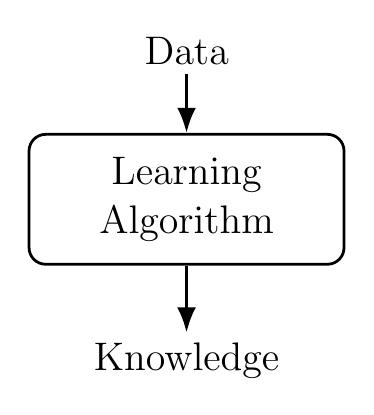
\begin{tikzpicture}[
				node distance=0.65cm,
				every node/.style={font=\Large},
				box/.style={
					draw=black,
					rounded corners=6pt,
					align=center,
					minimum width=4.0cm,
					minimum height=1.65cm,
					line width=1pt
				},
				arrow/.style={
					-{Latex[length=3.2mm]},
					line width=1.1pt
				}
				]
				\node (data) {Data};
				\node[box,below=0.75cm of data] (alg)
				{Learning\\Algorithm};
				\node[below=0.85cm of alg] (knowledge)
				{Knowledge};
				
				\draw[arrow] (data) -- (alg);
				\draw[arrow] (alg) -- (knowledge);
			\end{tikzpicture}
		\end{column}
		
	\end{columns}
\end{frame}
% -----------------------------------------------------------------------------
% 14. Rocket and fire emoji from the source title are omitted.
% -----------------------------------------------------------------------------
\begin{frame}[t]{Machine Learning is Trending}
  \vspace{0.65cm}
  {\large
  \begin{itemize}
    \setlength{\itemsep}{0.72cm}
    \item Everywhere --- wide application
    \vspace{0.2cm}
      \begin{itemize}
        \item Finance, data scientist, medical diagnosis, translation, self-driving....
      \end{itemize}
    \item Foundation of artificial intelligence --- one of the most important
          technology for the society in the next 10s of years
          \vspace{0.2cm}
      \begin{itemize}
        \item ChatGPT, large language model, large multimodal model
      \end{itemize}
  \end{itemize}
  }
\end{frame}

% -----------------------------------------------------------------------------
% 15. The example images under each category are intentionally omitted.
% -----------------------------------------------------------------------------
\begin{frame}{Machine Learning Paradigms}
	
	{\large
\begin{itemize}
	\setlength{\itemsep}{0.72cm}
	\item Supervised learning
	
	\item Unsupervised learning
	
	\item Self-supervised learning
	
	\item Reinforcement learning
\end{itemize}
}

\end{frame}

% -----------------------------------------------------------------------------
% 16
% -----------------------------------------------------------------------------
\SectionSlide{Supervised Learning}

% -----------------------------------------------------------------------------
% 17. Scatter plot and annotations are intentionally omitted.
% -----------------------------------------------------------------------------
\begin{frame}[t]{Housing Price Prediction}
  \vspace{0.45cm}
  {\Large
  \begin{itemize}
    \setlength{\itemsep}{0.62cm}
    \item Given: a dataset that contains $n$ samples
  \end{itemize}
  }
  \vspace{-0.15cm}
  \[
    \bigl(x^{(1)},y^{(1)}\bigr),\ldots,
    \bigl(x^{(n)},y^{(n)}\bigr)
  \]
  {\Large
  \begin{itemize}
    \item Task: if a residence has $x$ square feet, predict its price?
  \end{itemize}
  }
  \SourceNote{Example from Stanford CS229}
\end{frame}

% -----------------------------------------------------------------------------
% 18. Fitted curves and scatter plot are intentionally omitted.
% -----------------------------------------------------------------------------
\begin{frame}[t]{Housing Price Prediction}
	\vspace{0.45cm}
	

	
	\begin{center}
		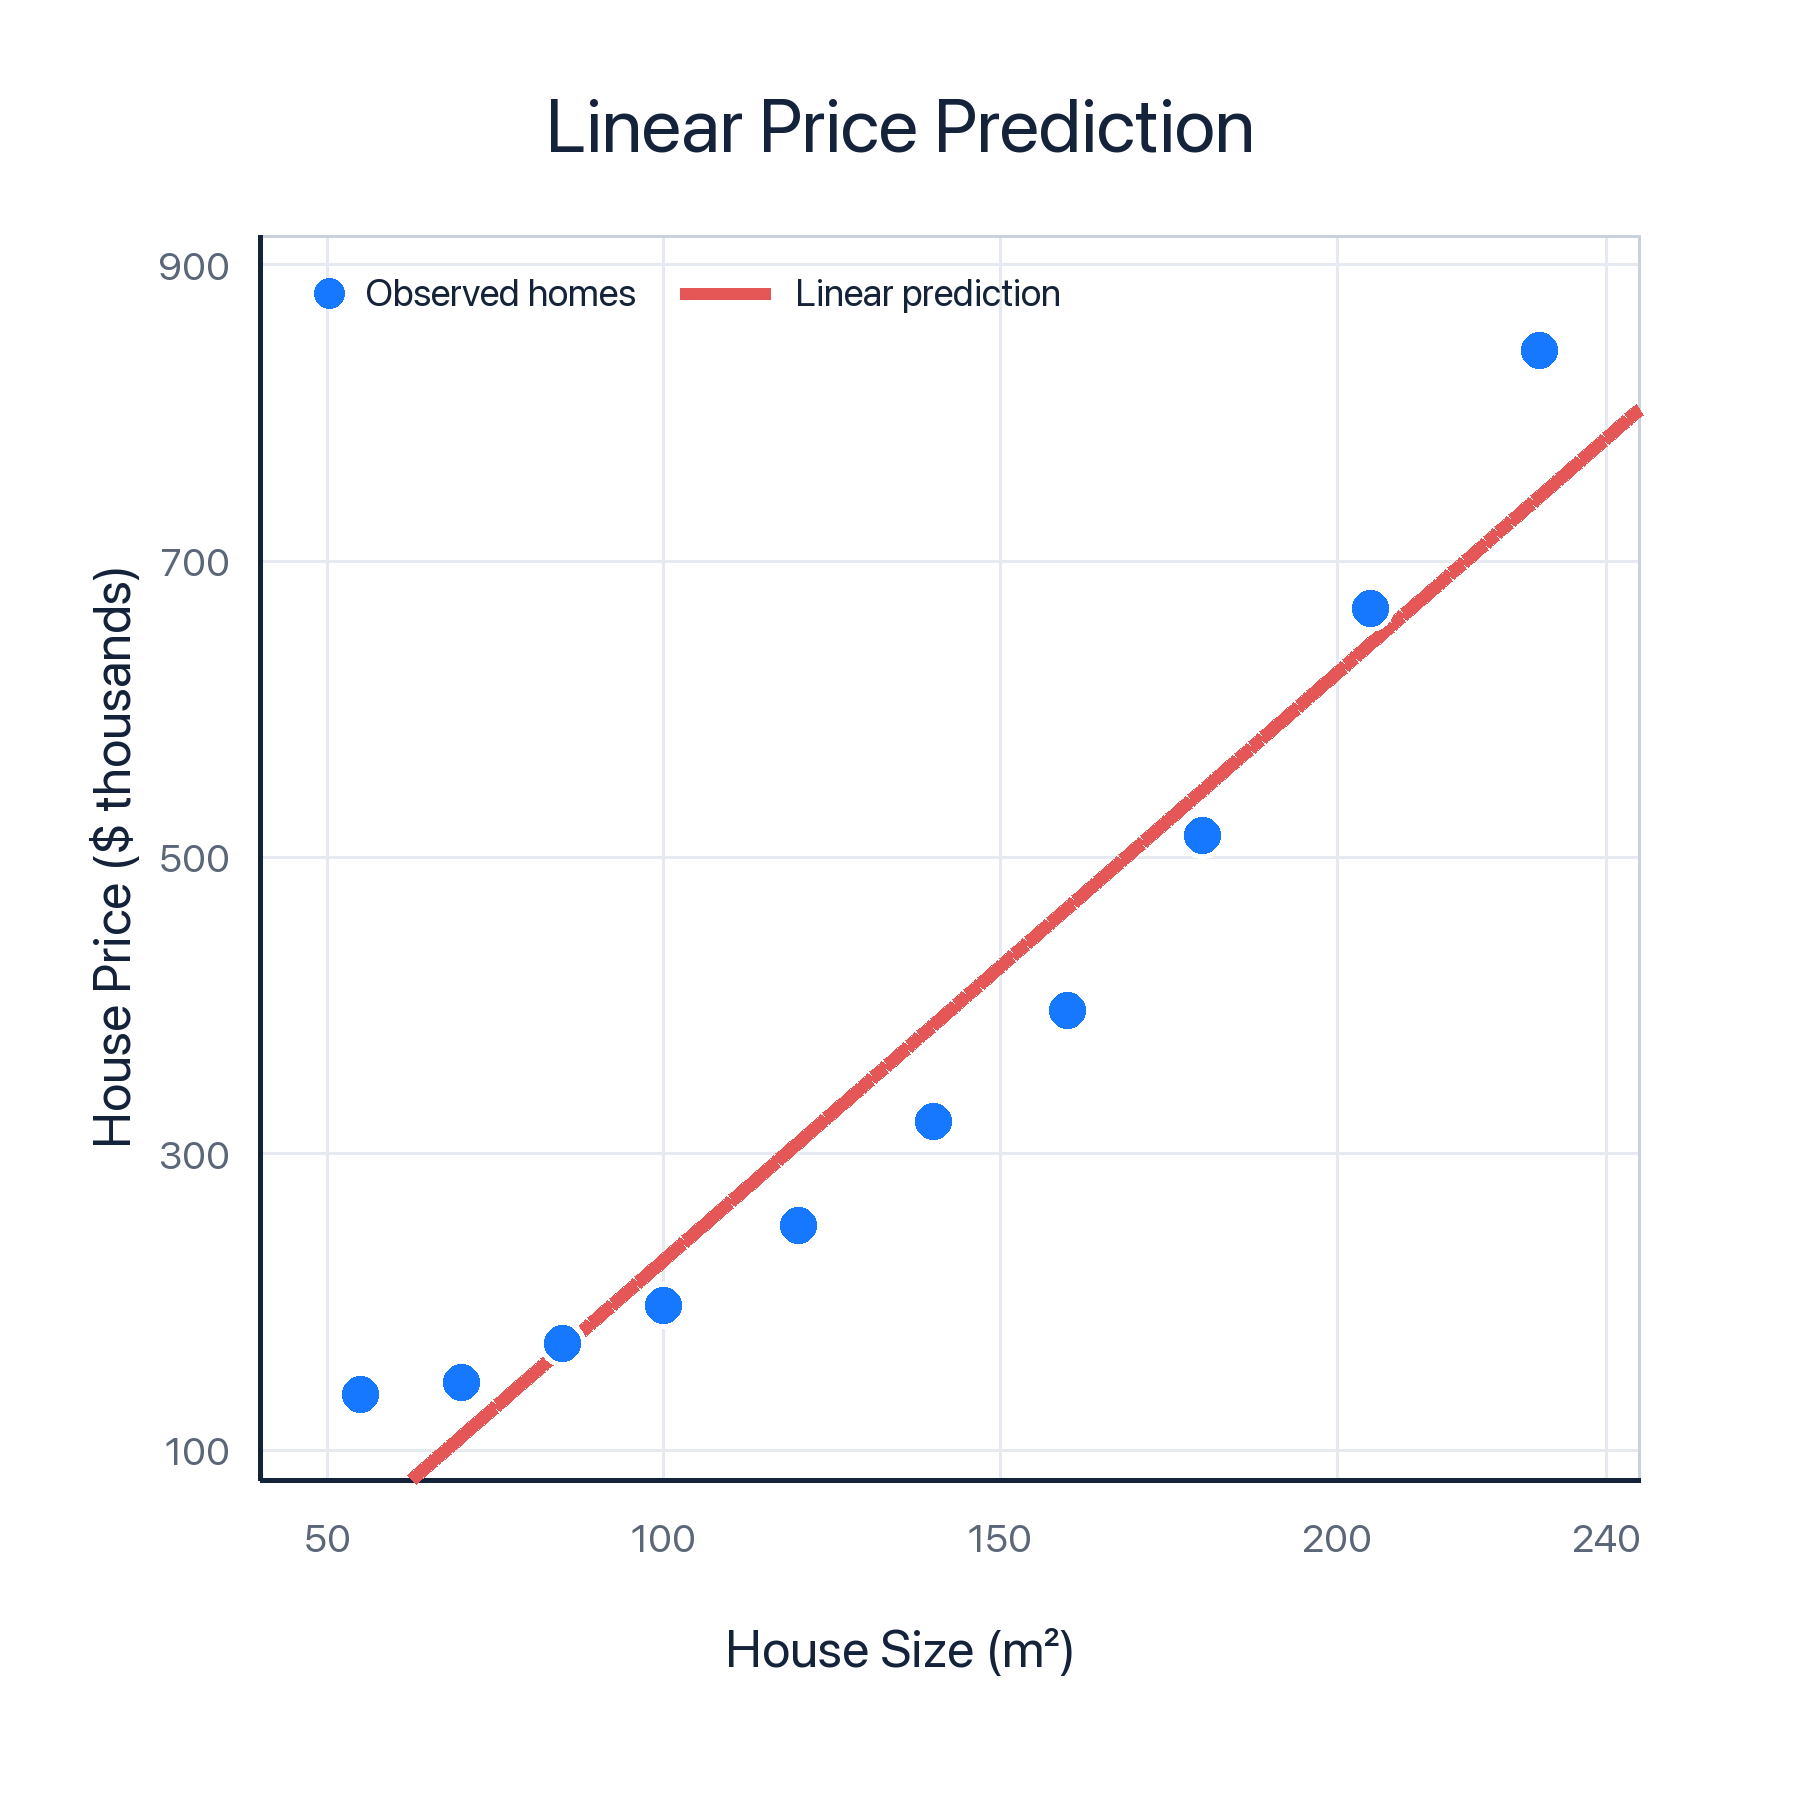
\includegraphics[
		width=0.8\textwidth,
		height=0.8\textheight,
		keepaspectratio
		]{image/housing-price-linear.png}
		\hspace{0.5cm}
		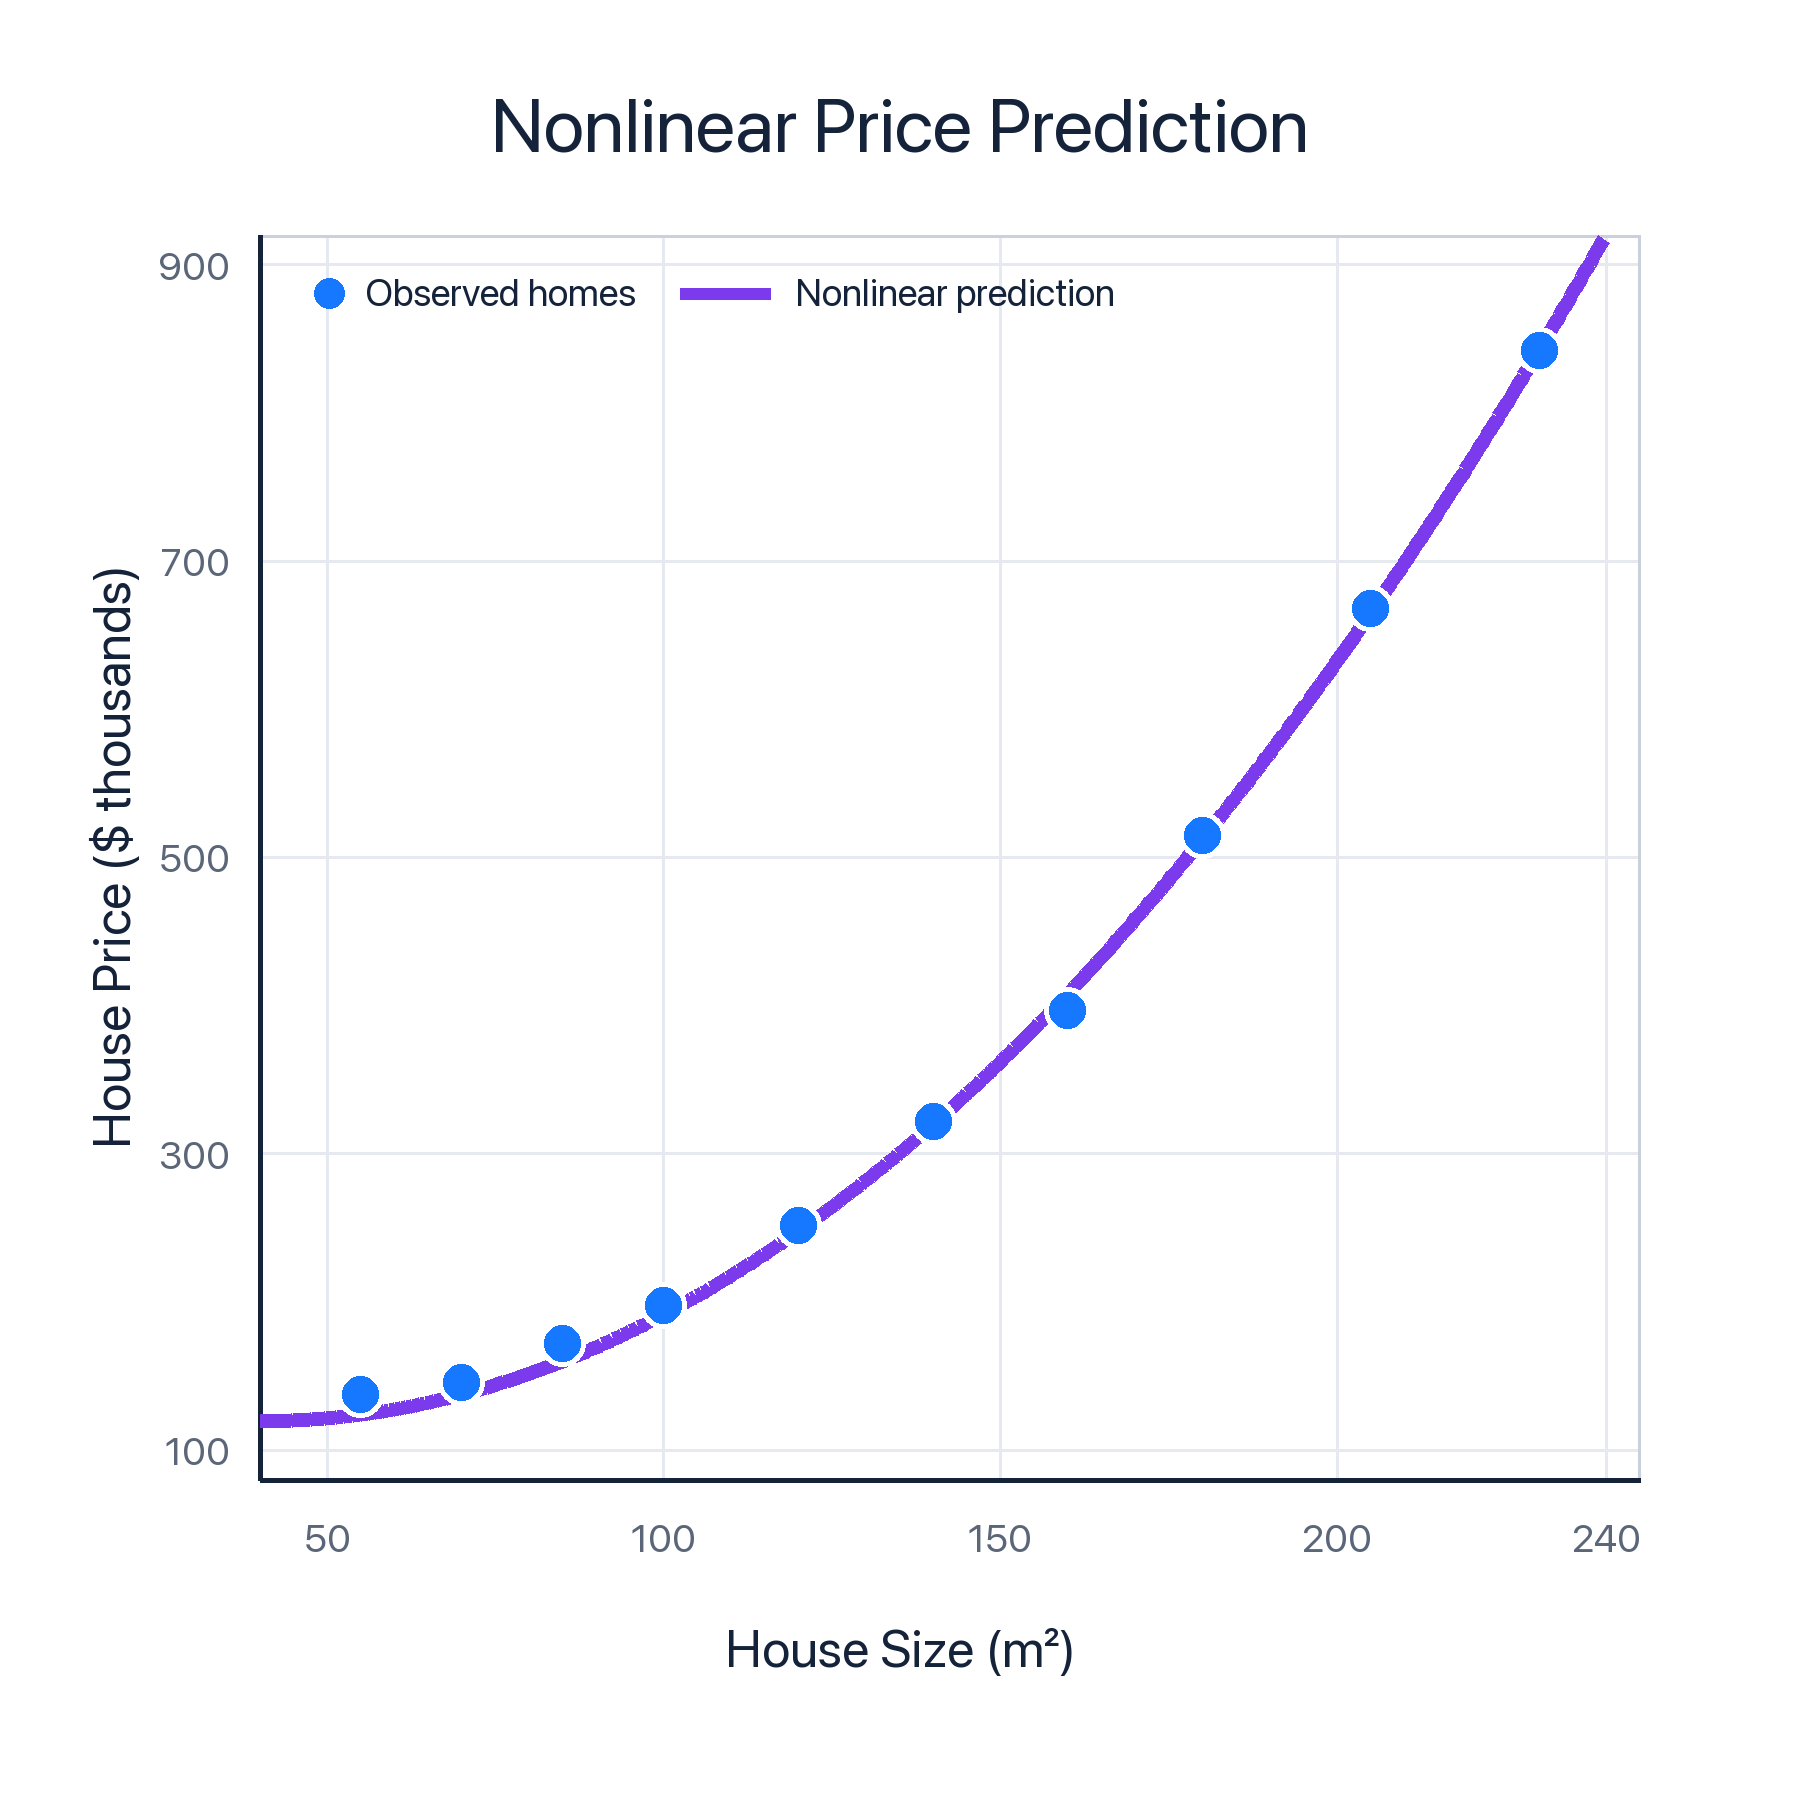
\includegraphics[
		width=0.8\textwidth,
		height=0.8\textheight,
		keepaspectratio
		]{image/housing-price-nonlinear.png}
	\end{center}
\end{frame}

% -----------------------------------------------------------------------------
% 19. Plot is intentionally omitted.
% -----------------------------------------------------------------------------
\begin{frame}[t]{More Features}
  \vspace{0.65cm}
  {\Large
  \begin{itemize}
    \item Suppose we also know the lot size
  \end{itemize}
  }
  \SourceNote{Example from Stanford CS229}
\end{frame}

% -----------------------------------------------------------------------------
% 20. 3D plot is intentionally omitted.
% -----------------------------------------------------------------------------
\begin{frame}[t]{More Features}
  \vspace{0.35cm}

\begin{columns}[T,onlytextwidth]
	
	% Left side: text and equation
	\begin{column}{0.56\textwidth}
		\vspace{0pt}
		
		{\large
			\begin{itemize}
				\setlength{\itemsep}{0.65cm}
				\item Suppose we also know the lot size
				\item Task: find a function that maps
			\end{itemize}
		}
		
		\vspace{0.35cm}
		
		% Resize the equation so it fits inside the left column
	{\hspace{2cm}
			$\displaystyle
			\underbrace{(\text{size},\text{ lot size})}_{
				\substack{\text{features/input}\\x\in\mathbb{R}^2}}
			\quad\longrightarrow\quad
			\underbrace{\text{price}}_{
				\substack{\text{label/output}\\y\in\mathbb{R}}}
			$
		}
	\end{column}
	
	\hspace{0.02\textwidth}
	
	% Right side: image
	\begin{column}{0.42\textwidth}
		\vspace{20pt}
		\hfill
		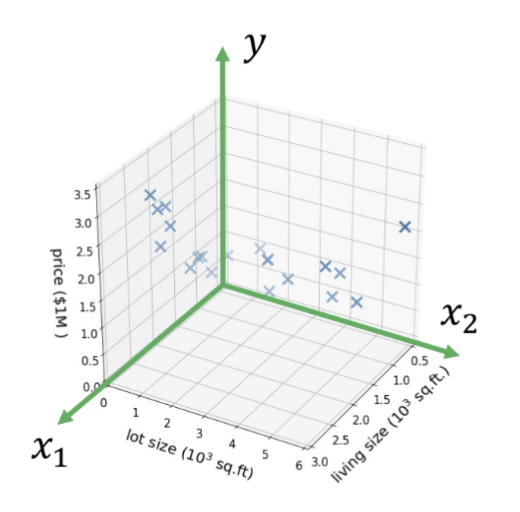
\includegraphics[
		width=0.8\linewidth,
		height=0.8\textheight,
		keepaspectratio
		]{image/housing-price-3d.png}
	\end{column}
	
\end{columns}
  
\end{frame}


\begin{frame}[t]{More Features}
	\vspace{0.35cm}
	
	\begin{columns}[T,onlytextwidth]
		
		% Left side: text and equation
		\begin{column}{0.56\textwidth}
			\vspace{0pt}
			
			{\large
				\begin{itemize}
					\setlength{\itemsep}{0.65cm}
					\item Suppose we also know the lot size
					\item Task: find a function that maps
				\end{itemize}
			}
			
			\vspace{0.35cm}
			
			% Resize the equation so it fits inside the left column
			{\hspace{2cm}
				$\displaystyle
				\underbrace{(\text{size},\text{ lot size})}_{
					\substack{\text{features/input}\\x\in\mathbb{R}^2}}
				\quad\longrightarrow\quad
				\underbrace{\text{price}}_{
					\substack{\text{label/output}\\y\in\mathbb{R}}}
				$
			}
			  \vspace{-0.05cm}
			{\large
				\begin{itemize}
					\item Dataset:  \small $(x^{(1)}, y^{(1)}), ... , (x^{(n)}, y^{(n)})$
				\end{itemize}
			}
			\[
			\text{where }\quad x^{(i)}=\bigl(x_1^{(i)},x_2^{(i)}\bigr)
			\]
		\end{column}
		
		\hspace{0.02\textwidth}
		
		% Right side: image
		\begin{column}{0.42\textwidth}
			\vspace{20pt}
			\hfill
			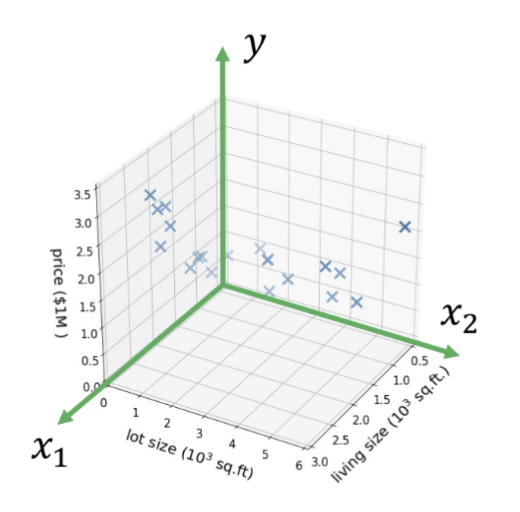
\includegraphics[
			width=0.8\linewidth,
			height=0.8\textheight,
			keepaspectratio
			]{image/housing-price-3d.png}
		\end{column}
		
	\end{columns}
	
\end{frame}
% -----------------------------------------------------------------------------
% 21. 3D plot is intentionally omitted.
% -----------------------------------------------------------------------------
% -----------------------------------------------------------------------------
% 22
% -----------------------------------------------------------------------------
\begin{frame}{High-dimensional Features}
  \centering
  \vspace{0.40cm}
  {\fontsize{18}{21}\selectfont
  \[
  x=
  \begin{bmatrix}
    x_1\\
    x_2\\
    x_3\\
    \vdots\\
    \vdots\\
    x_d
  \end{bmatrix}
  \quad
  \begin{array}{l}
    \text{--- living size}\\
    \text{--- lot size}\\
    \text{--- \# floors}\\
    \text{--- condition}\\
    \text{--- zip code}\\
    \vdots
  \end{array}
  \quad\longrightarrow\quad
  y\;\text{--- price}
  \]
  }
\end{frame}

% -----------------------------------------------------------------------------
% 23. Classification plot is intentionally omitted.
% -----------------------------------------------------------------------------
\begin{frame}[t]{Regression vs Classification}
  \vspace{0.55cm}
  {\large
  \begin{itemize}
    \setlength{\itemsep}{0.62cm}
    \item Regression: if $y\in\mathbb{R}$ is a continuous variable
  %  \vspace{0.2cm}
      \begin{itemize}
        \item E.g., price prediction
      \end{itemize}
    \item Classification: the label is a discrete variable
 %   \vspace{0.2cm}
      \begin{itemize}
        \item E.g., predicting the types of residence
      \end{itemize}
  \end{itemize}
  }
  \vspace{0.1cm}
  \centering
  	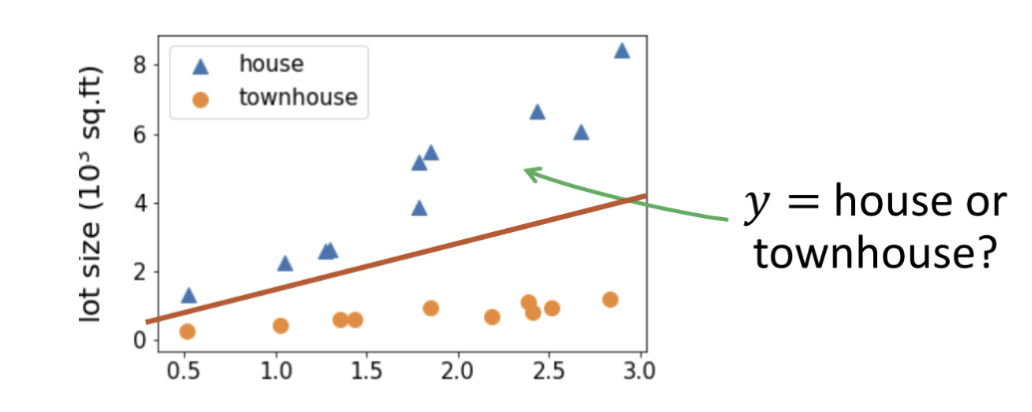
\includegraphics[
  width=0.55\linewidth,
  keepaspectratio
  ]{image/house_or_thouse.png}
\end{frame}


\SectionSlide{Unsupervised Learning}




\begin{frame}{Unsupervised Learning}
	\vspace{0.55cm}
{\large
	\begin{itemize}
		\setlength{\itemsep}{0.2cm}
		\item The dataset contains no labels:
		\quad $x^{(1)},\ldots,x^{(n)}$
		\item The goal is typically vague: find interesting structures in the data
	\end{itemize}
}
\vspace{0.1cm}

\centering
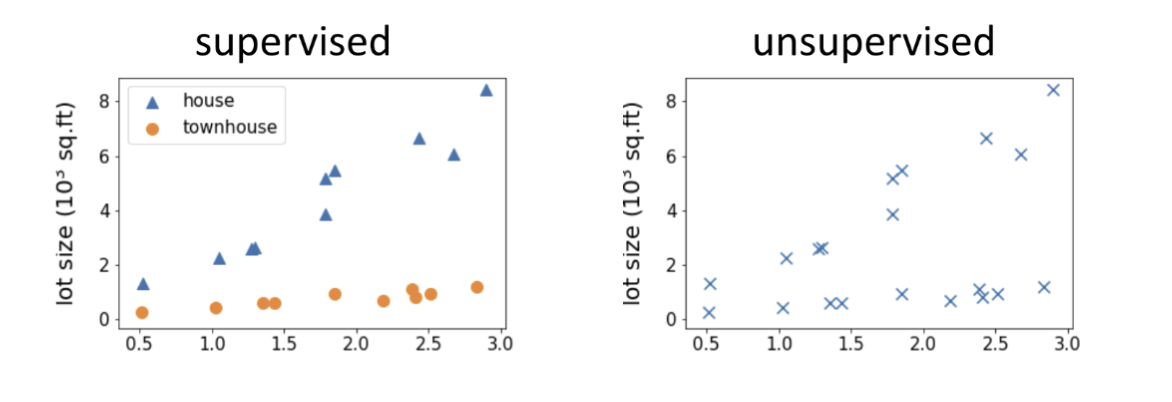
\includegraphics[
width=0.75\linewidth,
keepaspectratio
]{image/s_us_com.png}

\hfill \scriptsize Examples from CS229
\end{frame}



\begin{frame}{Clustering}
		\vspace{0.55cm}
\centering
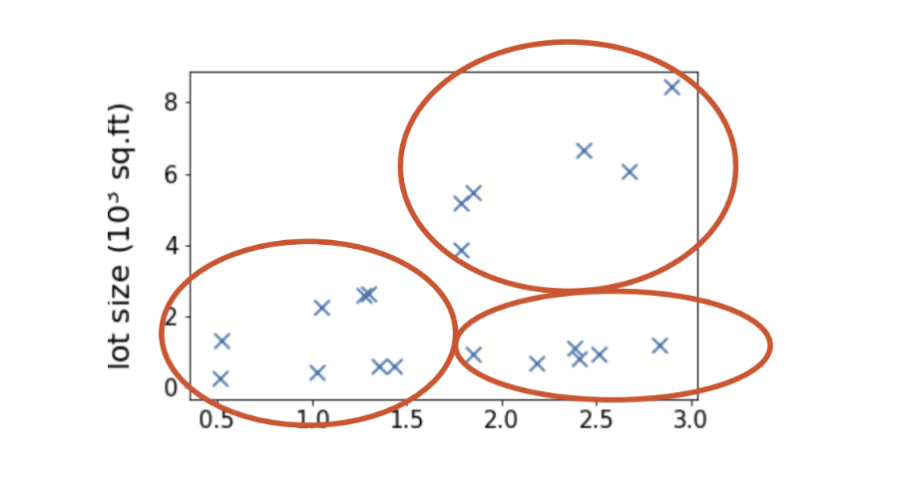
\includegraphics[
width=0.75\linewidth,
keepaspectratio
]{image/clustering.png}
\end{frame}


\begin{frame}{Word Embeddings}

		\vspace{0.55cm}
\centering

\includegraphics[
width=0.75\linewidth,
keepaspectratio
]{image/wtv.png}
\end{frame}



\SectionSlide{Self-supervised Learning}


\begin{frame}{Language Models}
  \centering
  \vspace{0.20cm}
  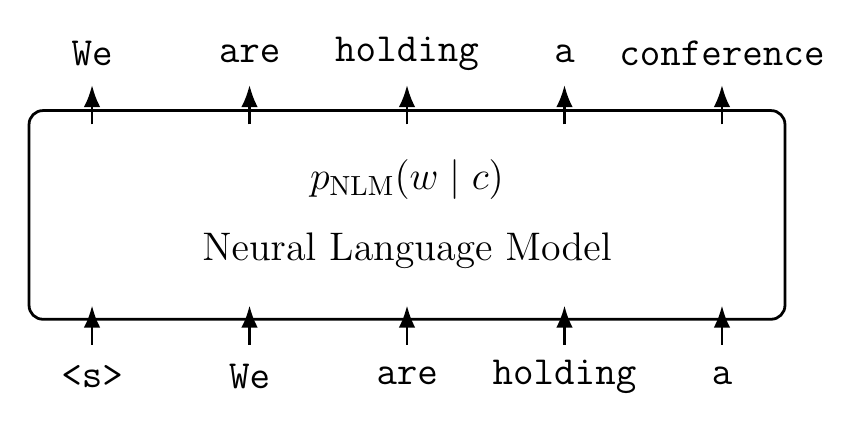
\begin{tikzpicture}[>=Latex]
    \node[
      draw=black,
      rounded corners=5pt,
      line width=1pt,
      minimum width=9.6cm,
      minimum height=2.65cm,
      align=center
    ] (model) at (0,0) {};

    \node[font=\Large] at (0,0.45) {$p_{\mathrm{NLM}}(w\mid c)$};
    \node[font=\Large] at (0,-0.45) {Neural Language Model};

    \foreach \x/\token in {-4/{<s>},-2/{We},0/{are},2/{holding},4/{a}} {
      \node[font=\Large\ttfamily] at (\x,-2.05) {\token};
      \draw[-{Latex[length=2.8mm]},line width=1pt] (\x,-1.65) -- (\x,-1.15);
    }

    \foreach \x/\token in {-4/{We},-2/{are},0/{holding},2/{a},4/{conference}} {
      \node[font=\Large\ttfamily] at (\x,2.05) {\token};
      \draw[-{Latex[length=2.8mm]},line width=1pt] (\x,1.15) -- (\x,1.65);
    }
  \end{tikzpicture}
  
  The label is from the data itself. 
\end{frame}

% -----------------------------------------------------------------------------
% 32. Prompt/completion screenshot is intentionally omitted.
% -----------------------------------------------------------------------------
\begin{frame}{Large Language Models}
	
	  \vspace{0.15cm}
	
		An autoregressive model predicts each token using only the
		tokens that appear before it:
		\[
		P(x_1,\ldots,x_T)
		=
		\prod_{t=1}^{T} P(x_t\mid x_1,\ldots,x_{t-1}).
		\]
	
	\vspace{-0.2cm}
	
	\begin{columns}[T,onlytextwidth]
		
		\begin{column}{0.53\textwidth}
			\begin{exampleblock}{Training examples}
				\small
				\begin{tabular}{ll}
					\textbf{Input context} & \textbf{Target}\\[0.12cm]
					\texttt{The}              & \texttt{cat}\\
					\texttt{The cat}          & \texttt{sat}\\
					\texttt{The cat sat}      & \texttt{on}\\
					\texttt{The cat sat on}   & \texttt{the}\\
					\texttt{The cat sat on the} & \texttt{mat}
				\end{tabular}
			\end{exampleblock}
		\end{column}
		
		\begin{column}{0.43\textwidth}
			\begin{exampleblock}{Generation}
				\small
				\texttt{Machine}\\
				$\longrightarrow$ \texttt{Machine learning}\\
				$\longrightarrow$ \texttt{Machine learning can}\\
				$\longrightarrow$ \texttt{Machine learning can predict}\\
				$\longrightarrow \cdots$
			\end{exampleblock}
		\end{column}
		
	\end{columns}
	

\end{frame}

% -----------------------------------------------------------------------------
% 33. In-context learning examples are intentionally omitted.
% -----------------------------------------------------------------------------

% -----------------------------------------------------------------------------
% 34
% -----------------------------------------------------------------------------
\SectionSlide{Reinforcement Learning}

% -----------------------------------------------------------------------------
% 35. AlphaGo image is intentionally omitted.
% -----------------------------------------------------------------------------
\begin{frame}{AlphaGo}
			\vspace{0.55cm}
	\centering
	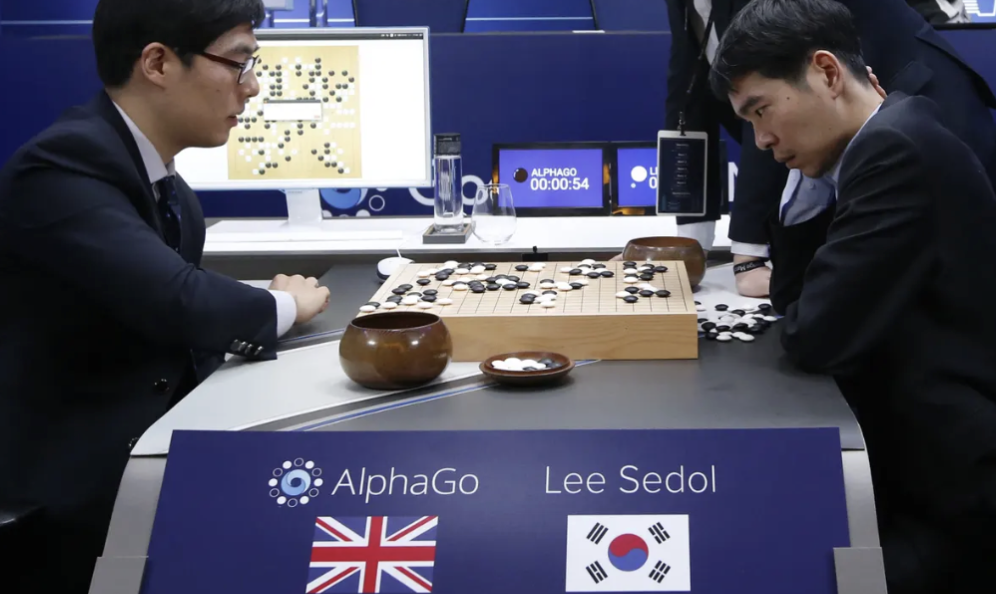
\includegraphics[
	width=0.8\linewidth,
	height = 0.6\linewidth,
	keepaspectratio
	]{image/alphago.png}
\end{frame}

% -----------------------------------------------------------------------------
% 36. Atari Breakout image is intentionally omitted.
% -----------------------------------------------------------------------------
\begin{frame}{Atari Breakout Game}
				\vspace{0.55cm}
	\centering
	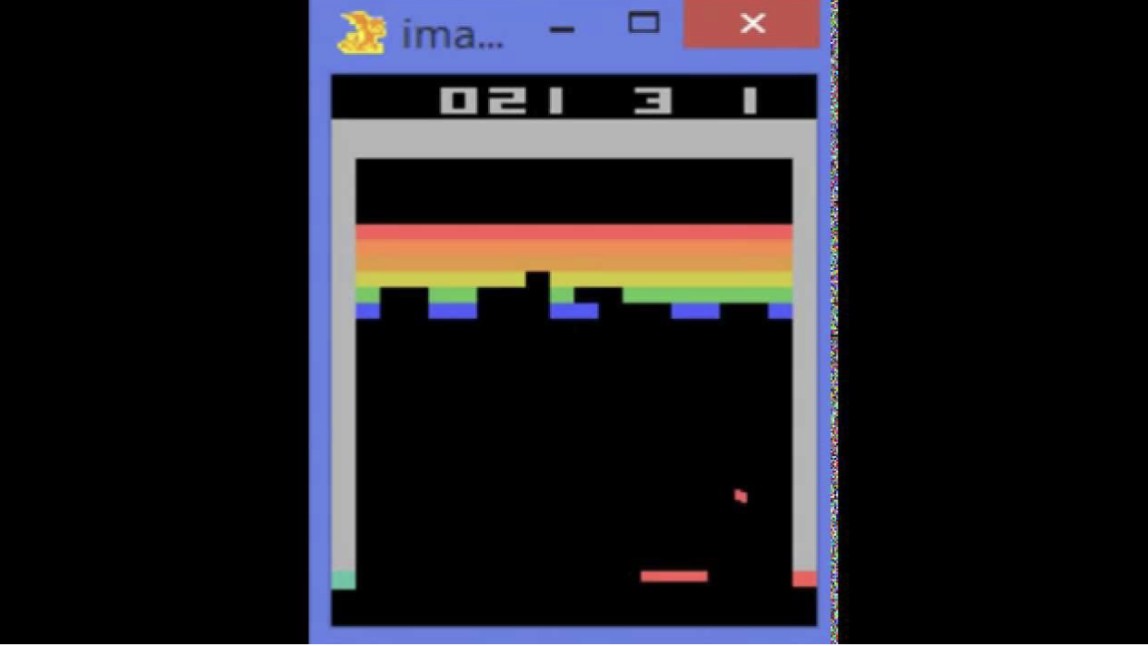
\includegraphics[
	width=0.8\linewidth,
	keepaspectratio
	]{image/atari.png}
\end{frame}

% -----------------------------------------------------------------------------
% 37. Robot and maze images are omitted; the interaction loop is kept.
% -----------------------------------------------------------------------------
\begin{frame}[t]{Reinforcement Learning}
	\vspace{0.2cm}
  \begin{itemize}
  	\item \large RL can collect data \textcolor{blue}{interactively}
  \end{itemize}
  \vspace{0.2cm}
	\centering
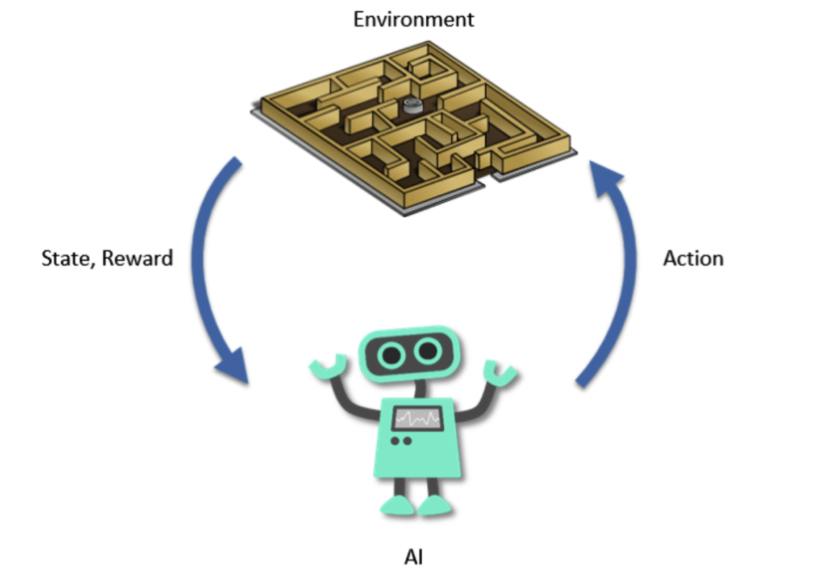
\includegraphics[
width=0.6\linewidth,
keepaspectratio
]{image/rl.png}
\end{frame}


\begin{frame}[t]{Other Learning Paradigms}
	
	
	
	
\end{frame}

% -----------------------------------------------------------------------------
% 38
% -----------------------------------------------------------------------------
\begin{frame}[t]{Overview of Topics}
  \vspace{-0.18cm}
  \renewcommand{\arraystretch}{1.08}
  \begin{columns}[T,onlytextwidth]
    \column{0.465\textwidth}
      \scriptsize
      \begin{tabular}{|>{\raggedright\arraybackslash}p{0.93\linewidth}|}
        \hline
        Introduction \\ \hline
        Math basics \\ \hline
        Foundations of machine learning \\ \hline
        Linear/Logistic regression \\ \hline
        Generalized linear models, classification \\ \hline
        Kernel methods \\ \hline
        SVM \\ \hline
        MLE\\ \hline
        Gradient descent, SGD, Newton's method \\ \hline
        Generalization, bias-variance tradeoff \\ \hline
        Clustering \\ \hline
        Expectation Maximization \\ \hline
        PCA/ICA \\ \hline
        mid-term exam \\ \hline
    %    Probabilistic Graphical Models \\ \hline
    %    HMM \\ \hline
      \end{tabular}

    \column{0.475\textwidth}
      \vspace{0.95cm}
      \scriptsize
      \begin{tabular}{|>{\raggedright\arraybackslash}p{0.93\linewidth}|}
        \hline
        Basics of FNN\\ \hline
        Neural networks architectures (CNN/RNN) \\ \hline
        Variational autoencoder \\ \hline
        Generative adversarial networks \\ \hline
        Stable diffusion \\ \hline
        Reinforcement Learning \\ \hline
        Large language models \\ \hline
      \end{tabular}
  \end{columns}
\end{frame}

% -----------------------------------------------------------------------------
% 39
% -----------------------------------------------------------------------------
\begin{frame}
  \centering
  \vfill
  {\color{slideorange}\fontsize{31}{38}\selectfont\bfseries
    Thank You!\par
    \vspace{1.5cm}
    Questions?
  }
  \vfill
\end{frame}

\end{document}
